\section{Results}
\begin{figure}[b]
  \centering
   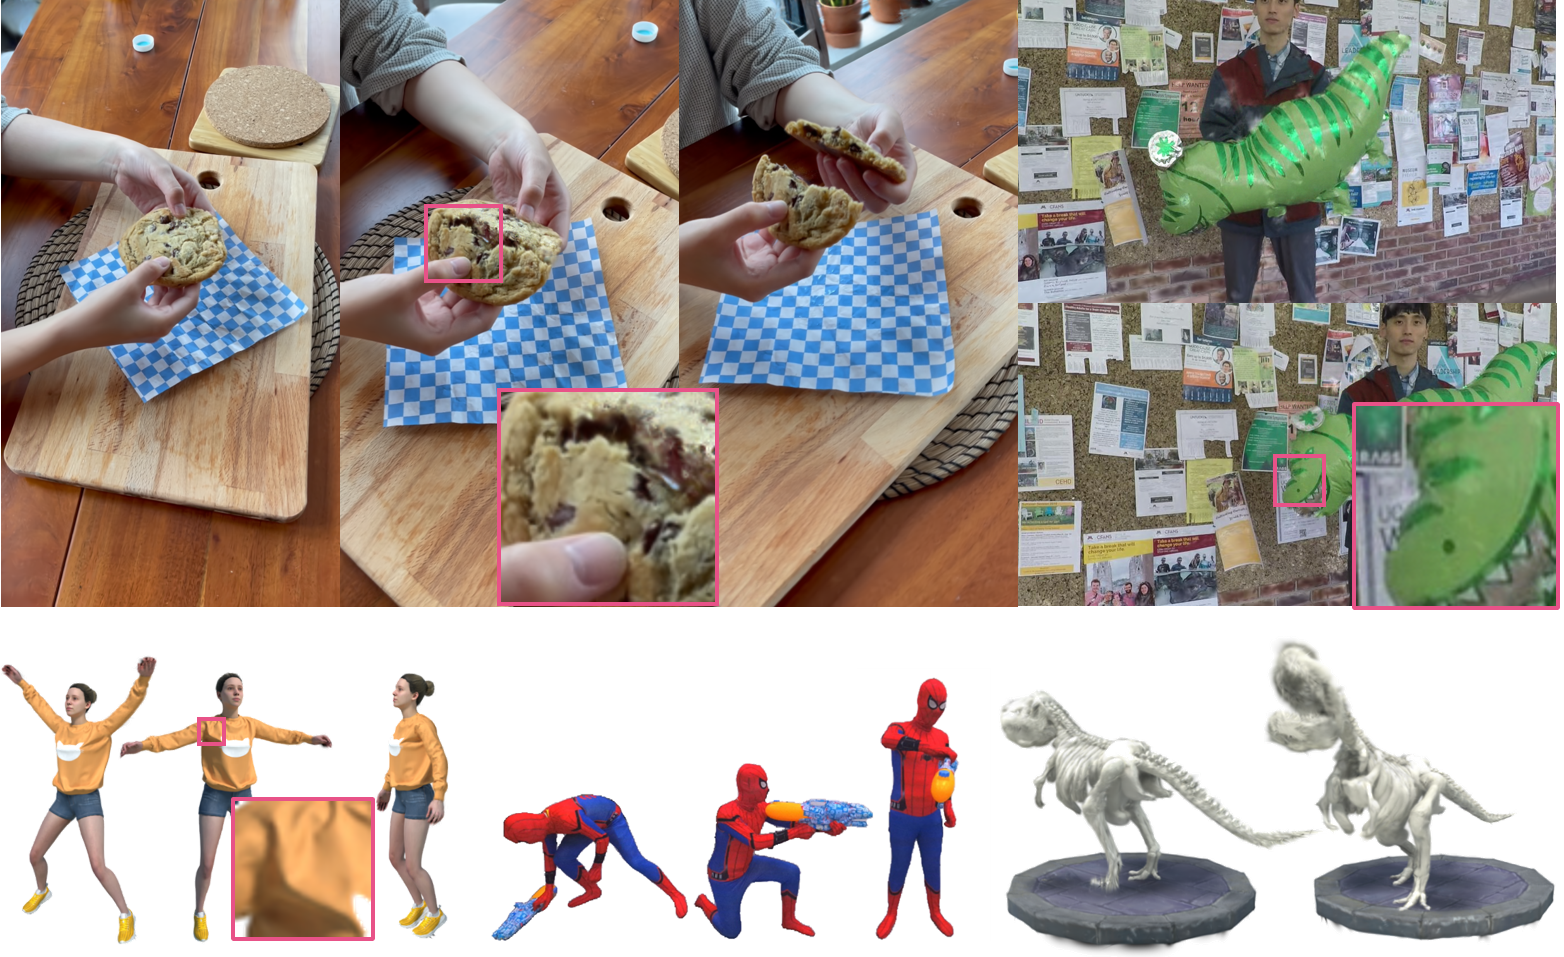
\includegraphics[width=1.0\linewidth]{sec/fig/results.png}

   \caption{The results of our method}
   \label{fig:results}
\end{figure}
The picture presented as Fig.~\ref{fig:results} demonstrates the effectiveness of our method. The top-left data originates from the HyperNeRF Dataset, with the camera setting being a pinhole camera model with tangential and radial distortion. The data in the top right is from the Dynamic Scene Dataset, captured using a moving monocular camera; it represents short-term dynamic events ($\sim$ 5 seconds) recorded with a hand-held, moving camera. The bottom-left and bottom-right data are from D-Nerf, with the camera setting being a sparse set of images of a dynamic scene, captured by a monocular camera for sparse views by moving non-rigidly. Lastly, the data in the center bottom is from the Instant-NVR dataset, captured with an RGBD Kinect camera.

\section{Limitations}
Our method still has some limitations. The DynTCG takes RGBD images as input, which requires an RGBD camera to capture. Though we could use monodepth to estimate depth from RGB images, the error in depth estimation can lead to a bad effect on the back-projection module. Besides, our optical flow tracking will fail to deal with a non-continuous image input, limiting the data set to continuous captures. 

\section{Conclusions}
We have presented a deformable Gaussian representation that takes monocular RGBD input and synthesizes a dynamic novel view. By utilizing optical flow tracking from 2D images into deformable dynamic Gaussian-splatting, our approach achieves high-fidelity rendering results, outperforming previous methods in terms of quality, training speed, and storage. Our optical flow and Gaussian point cloud wrap method provides a favorable prior, achieving a great acceleration on the deformable network training speed. We also present a residual encoding method to address the long sequence storage problem, by applying quantization and RANS Encoding on the residual point cloud, we achieve a compression rate of 25, making long dynamic sequences loading and training. Our experimental results show that our method outperforms other monocular methods under the same settings. We believe our method achieves a critical step in monocular dynamic novel view synthesis. 


\section{Acknowledgement and Contribution}
% \begin{enumerate}
%     \item Baseline (the development of D-net) (Hong Yu, Shen Zhehao)
%     \item Apply flow tracking as a powerful prior to D-net (Shen Zhehao)
%     \item Modify the D-net (remove the scale and improve the training speed) (Zhou Shouchen)
%     \item Use the Quantization and RANS Encoding to compress Gaussians (Wang Penghao)
%     \item Residual compression design (Wang Penghao, Zhang Zhirui)
%     \item Dynamic viewer development (Zhang Zhirui)
%     \item Comparison experiment (Shen Zhehao, Hong Yu, Zhang Zhirui, Wang Penghao, Zhou Shouchen)
%     \item Ablation experiment (Shen Zhehao, Wang Penghao, Zhou Shouchen)
%     \item Poster design (Hong Yu)
% \end{enumerate}
% % 此外,我们在Yuheng Jiang的帮助下在对比实验中跑通了instant-nvr的结果,感谢他的帮助
We extend our gratitude to Yuheng Jiang for his assistance with the implementation of the Instant-NVR results in comparison experiments.

The contributions to this work are as follows: Yu Hong and Zhehao Shen developed the initial baseline through the design of the deform net. Zhehao Shen further enhanced this by integrating flow tracking as an effective prior. Shouchen Zhou contributed significant improvements to the deform net by removing redundant scale parameters and optimizing training speed. Penghao Wang introduced a novel approach to Gaussian compression using Quantization and RANS Encoding, as well as collaborating with Zhirui Zhang on the residual compression design. Zhirui Zhang also spearheaded the development of the dynamic viewer. Comparative and ablation experiments were conducted by Zhehao Shen, Yu Hong, Zhirui Zhang, Penghao Wang, and Shouchen Zhou, with Yu Hong taking the lead on poster design.

